\documentclass[aspectratio=169]{beamer}

\usetheme{Madrid}
\usecolortheme{seahorse}

\usepackage[utf8]{inputenc}
\usepackage[T1]{fontenc}
\usepackage{amsmath}
\usepackage{amssymb}
\usepackage{tikz}

\usetikzlibrary{arrows.meta, positioning}

\title{Iterated Averages in Practice}
\subtitle{A short talk for the OverBranch benchmark}
\author{OverBranch Benchmark Corpus}
\institute{Compiler Benchmark Suite}
\date{\today}

\begin{document}

\frame{\titlepage}

\begin{frame}{Outline}
  \tableofcontents
\end{frame}

\section{Motivation}

\begin{frame}{Why averages?}
  Averages are the simplest smoothing tools available:
  \begin{itemize}[<+->]
    \item They are cheap to compute.
    \item They reduce variance of noisy measurements.
    \item They are easy to explain to non-specialists.
  \end{itemize}
\end{frame}

\begin{frame}{Running mean}
  \begin{block}{Definition}
    For a sequence $(x_k)$, the running mean is
    \[
      \bar{x}_n = \frac{1}{n}\sum_{k=1}^{n} x_k .
    \]
  \end{block}
  \vspace{0.5em}
  The update rule can be written incrementally:
  \[
    \bar{x}_{n} = \bar{x}_{n-1} + \frac{x_n - \bar{x}_{n-1}}{n}.
  \]
\end{frame}

\section{Method}

\begin{frame}{Iterated averaging}
  \begin{itemize}
    \item<1-> Apply the two-point average $T$ once.
    \item<2-> Apply $T$ repeatedly to obtain a binomial kernel.
    \item<3-> The variance factor after $m$ steps is $\binom{2m}{m}4^{-m}$.
  \end{itemize}
\end{frame}

\begin{frame}{Pipeline}
  \centering
  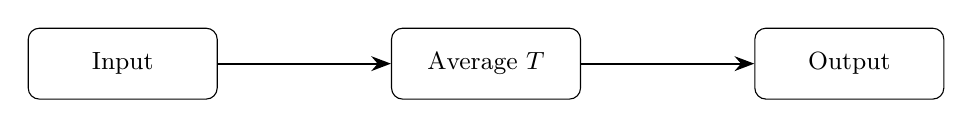
\begin{tikzpicture}[node distance=2.2cm, every node/.style={font=\small}]
    \node[draw, rounded corners, minimum width=2.4cm, minimum height=0.9cm] (in) {Input};
    \node[draw, rounded corners, minimum width=2.4cm, minimum height=0.9cm, right=of in] (avg) {Average $T$};
    \node[draw, rounded corners, minimum width=2.4cm, minimum height=0.9cm, right=of avg] (out) {Output};
    \draw[-{Stealth[length=2.5mm]}, thick] (in) -- (avg);
    \draw[-{Stealth[length=2.5mm]}, thick] (avg) -- (out);
  \end{tikzpicture}
\end{frame}

\section{Results}

\begin{frame}{Two columns}
  \begin{columns}[T]
    \begin{column}{0.48\textwidth}
      \textbf{Observations}
      \begin{itemize}
        \item Variance drops with $m$.
        \item Kernel weights are binomial.
      \end{itemize}
    \end{column}
    \begin{column}{0.48\textwidth}
      \textbf{Values}
      \begin{align*}
        m=1 &: \tfrac12 \\
        m=2 &: \tfrac38 \\
        m=3 &: \tfrac{5}{16}
      \end{align*}
    \end{column}
  \end{columns}
\end{frame}

\begin{frame}{Key facts}
  \begin{alertblock}{Caution}
    The closed form holds only for i.i.d.\ inputs.
  \end{alertblock}
  \begin{exampleblock}{Good news}
    Averaging is linear, so expectations are easy to propagate.
  \end{exampleblock}
\end{frame}

\begin{frame}{Enumerated points}
  \begin{enumerate}
    \item<1-> Define the operator.
    \item<2-> Compute its kernel.
    \item<3-> Verify the variance formula.
  \end{enumerate}
\end{frame}

\section{Conclusion}

\begin{frame}{Summary}
  \begin{itemize}
    \item Iterated averaging is a simple smoother.
    \item Its variance reduction is available in closed form.
  \end{itemize}
\end{frame}

\begin{frame}{Questions?}
  \centering
  Thank you for listening.
\end{frame}

\end{document}
